\subsection{Link nascosti}
Per rendere il sito pi\`u accessibile e migliorare la navigazione, in particolar modo per le persone non vedenti o comunque per tutti coloro che utilizzano come supporto uno screen reader, abbiamo deciso di introdurre numerosi link nascosti che consentono di muoversi agilmente all'interno di una determinata pagina web. \\
Ecco nel dettaglio la loro implementazione:
	\begin{itemize}
		\item \textbf{Salta men\`u di navigazione}: questo link ti permette di saltare il men\`u principale e posizionarti prima del breadcrumb in modo che l'utente possa ricordarsi dove si trova e poi leggere il contenuto della pagina. Questo aiuto ti informa anche che se salti quest'area della pagina salterai anche il link per accedere alla parte riservata all'amministrazione;
		\item \textbf{Salta contenuto}: questo collegamento serve se si ha la necessit\`a di andare alla sidebar perch\'e si vuole entrare in qualche sito correlato con il Circolo di Scherma o per visitare la Gallery per quanto riguarda la parte pubblica, mentre per la parte amministrativa ti consente di andare alla spiegazione di alcuni elementi per l'inserimento del testo nella form;
		\item \textbf{Torna su al men\`u di navigazione}: se si \`e letto tutto il contenuto o si ha superato la sidebar \`e possibile tornare al men\`u di navigazione per muoversi su altre pagine;
		\item \textbf{Torna al primo articolo/documento della pagina}: solo per le pagine che mostrano gli articoli e i documenti presenti \`e stata impostata una scorciatoia che ti permette di tornare al primo articolo/documento presente nel contenuto.
 
	\end{itemize}
Per tornare su all'inizio del contenuto per chi non utilizza screen reader \`e stato inserito un torna su unico situato in basso a destra che si attiva solo quando si \`e scorso la pagina.
\\ Il meccanismo viene gestito tramite javascript, ma se viene disabilitato allora vengono resi disponibili a tutti gli utenti le scorciatoie previste per i non vedenti. \\
\\ Per capire se i link siano stati inseriti in zone utili, abbiamo provato ad utilizzare il sito disabilitando gli stili. Inoltre ci siamo avvalsi del plugin Fangs per vedere come il sito viene visto da uno screen reader e ci\`o che appare sembra conforme alle necessit\`a di una persona con disabilit\`a in particolare visive.
\subsection{Lista nascosta}
Per facilitare la navigazione tra gli articoli e i documenti \`e stata inserita una lista nascosta di link (prima del contenuto) che rimandano al testo esatto selezionato.

\subsection{Tab Index}
Un altro meccanismo utilizzato per consentire una migliore esperienza per l'utente \`e stato quello di personalizzare i tab index in modo che ci si possa muovere pi\`u velocemente e senza avere bisogno del mouse.
In particolare gli abbiamo utilizzati per la navigazione nel men\`u e per i form presenti nella parte amministrativa.

\subsection{Breadcrumb}
Per far capire all'utente in che sezione del sito si trova, abbiamo pensato di modificare il colore di sfondo nella lista del menu\`per la pagina selezionata. La scelta di usare questo metodo  per veicolare questa informazione \`e stata scelta per eleganza, ma confermata da un'analisi del contrasto dei colori che rende ci\`o accessibile anche a chi ha particolari problemi di vista che analizzeremo nel capitolo successivo.
\\  Per chi utilizza screen reader è stato invece predisposto un campo nascosto che ti dice dove sei.
\\ Questo campo diventa visibile anche a tutti gli utenti quando si passa in modalità tablet e mobile in quanto il men\`u viene compresso e quindi non \`e pi\`u intuibile capire dove si \`e.

\subsection{Contrasti dei colori}
Per verificare che ci sia il giusto contrasto tra i colori applicati al sito abbiamo utilizzato due strumenti consigliati a lezione: Colour Contrast Analyser e Vischeck.
Abbiamo fatto due tipi di test, uno relativo al giusto contrasto tra il testo e lo sfondo e uno riguardante le possibile difficolt\`a che possono riscontrare utenti affetti da alcune distorsioni visive su una generica pagina del sito.
	\subsubsection {Test - Contrasto testo e sfondo}
	Questo tipo di test \`e  stato effettuato con Colour Contrast Analyser e si riscontrano i seguenti risultati:
	\\ Il contrasto risultante del colore azzurro chiaro (ebffff) di sfondo e nero come testo ha superato tutti i test presenti nell'applicazione.
	\\ L'analisi della \textbf{differenza colore/luminosit\`a} per una visione normale da risultati (745/249) con soglia minima fissata per superare il test a 500. Anche per chi soffre di alcuni distrubi della vista* i test sono superati con un minimo margine, ma sufficiente a garantirne l'accessibilit\`a.
	\\ Anche l'analisi \textbf{della luminosit\`a} risulta positiva a tutte le prove con rapporto di contrasto 20.3:1, con soglia minima perchè tutti i test siano validi fissata a 7:1, per chi vede normalmente la pagina. Rimane un rapporto alto anche per chi soffre di alcuni disturbi della vista* compreso tra i (17.3 e 19.9):1.
	\\
	\\
	\\Il contrasto risultante del colore blu di sfondo e bianco come testo usato nel men\`u di navigazione ha superato tutti i test presenti nell'applicazione.
	\\ L'analisi della \textbf{differenza colore/luminosit\`a} per una visione normale da risultati (543/212) con soglia minima fissata per superare il test a 500. Anche per chi soffre di alcuni distrubi della vista* i test sono superati con un discreto margine.
	\\ Anche l'analisi \textbf{della luminosit\`a} risulta positiva a tutte le prove con rapporto di contrasto 10.9:1, con soglia minima perchè tutti i test siano validi fissata a 7:1, per chi vede normalmente la pagina. Rimane comunque a un buon rapporto compreso tra i (9.7 e 14.4):1 per chi soffre di alcuni disturbi della vista*.
	\\
	\\
	\\Sono stati analizzati anche i contrasti con i colori dei link (normale,visitato) con lo sfondo azzurrino.
	\\Per quanto riguarda questi link, sia l'analisi della differenza colore/luminosit\`a sia quella della luminosit\`a,  vengono superate. In alcuni casi e per alcune distorsioni con una soglia minima, mentre per altri con un ampio margine.
	\\ \\ \textbf{*Disturbi della vista testati}: daltonismo, protanopia, tritanopia, deuteranopia.

	\subsubsection {Test - Distorsioni visive}
	Il sequente test invece \`e  stato effettuato attraverso il sito web Vischeck e si riscontrano i seguenti risultati:
	\begin{itemize}
	\item Per chi soffre di \textbf{deuteranopia}, cio\`e chi confonde il rosso porpora con il verde, in figura \ref{deuteranopia} ci\`o che appare:
	
	\item Per chi soffre di \textbf{pronatopia}, cio\'e una forma di daltonismo per i colori rosso e verde,  in figura \ref{protanopia} ci\`o che appare:
	
	\item Per chi soffre di \textbf{tritanopia}, cio\`e cecit\`a per il blu e il violetto, in figura \ref{tritanopia} ci\`o che appare:
	\end{itemize}
	
	\begin{figure}[h!]
		\centering
		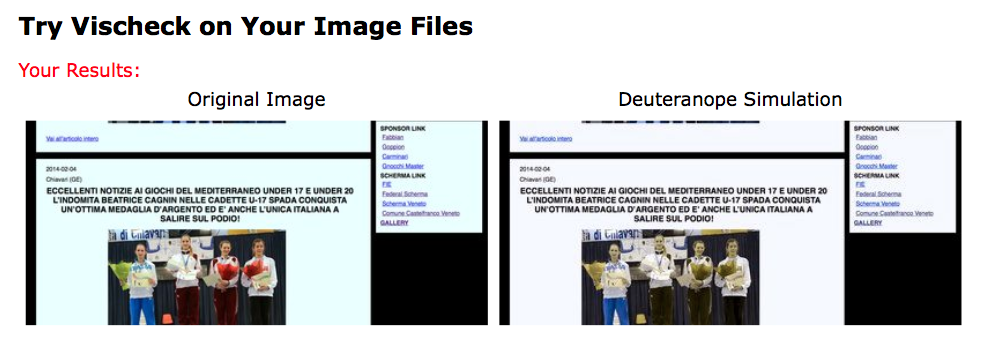
\includegraphics[scale=0.4]{images/contrasto_pagina_deuteranope.png}
		\caption{Visualizzazione sito per chi soffre di deuteranopia}
		\label{deuteranopia}
	\end{figure}	
	
	\begin{figure}[h!]
		\centering
		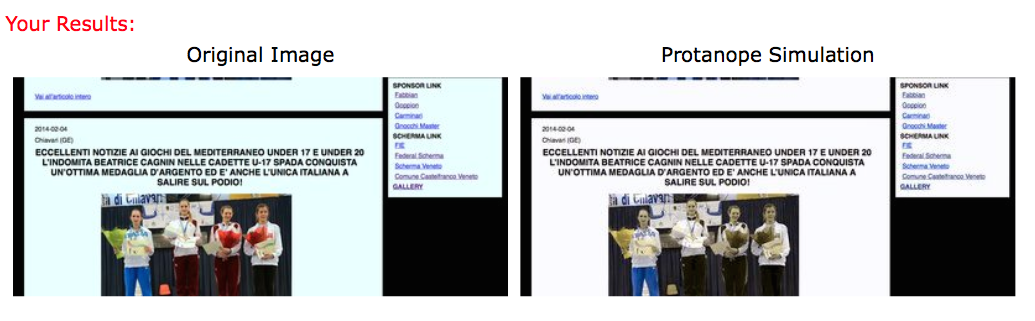
\includegraphics[scale=0.4]{images/contrasto_pagina_protanope.png}
		\caption{Visualizzazione sito per chi soffre di protanopia}
		\label{protanopia}
	\end{figure}
	
	\begin{figure}[h!]
		\centering
		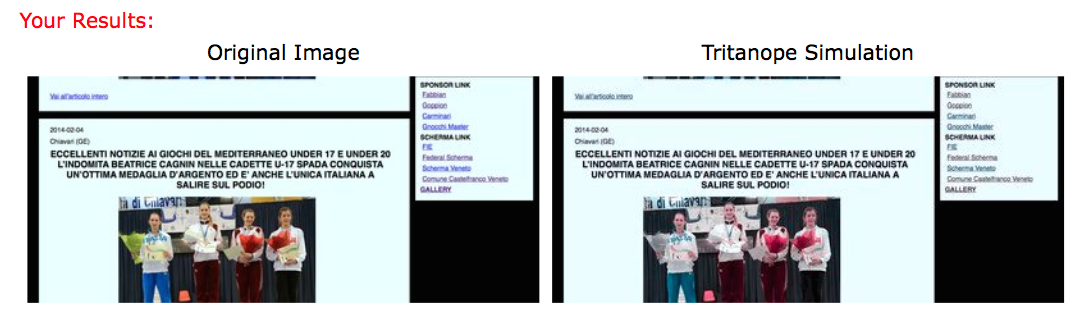
\includegraphics[scale=0.4]{images/contrasto_pagina_tritanope.png}
		\caption{Visualizzazione sito per chi soffre di tritanopia}
		\label{tritanopia}
	\end{figure}
	\newpage
	\textbf{Conclusioni}: per tutti e tre i tipi di distorsione il contrasto che si ottiene fa si che l'utente riesca comunque a comprendere il contenuto e a orientarsi nella pagina riuscendo ad interpretare il men\`u e i link presenti.

\subsection{Mappa del sito}
\`E stato scelto di non inserire una mappa in quanto il numero di pagine presenti nel sito \`e in numero ristretto e difficilmente l'utente potr\`a perdersi durante la navigazione.